\documentclass[12pt]{amsart}

\addtolength{\hoffset}{-2.25cm}
\addtolength{\textwidth}{4.5cm}
\addtolength{\voffset}{-2.5cm}
\addtolength{\textheight}{5cm}
\setlength{\parskip}{0pt}
\setlength{\parindent}{15pt}
\usepackage{pgfplots} % package used to implement the plot
\usepackage{amsthm}
\usepackage{amsmath}
\usepackage{amssymb}
\usepackage[colorlinks = true, linkcolor = black, citecolor = black, final]{hyperref}

\usepackage{graphicx}
\usepackage{multicol}
\usepackage{ marvosym }
\usepackage{wasysym}
\usepackage{tikz}
\usetikzlibrary{patterns}

\newcommand{\ds}{\displaystyle}

\setlength{\parindent}{0in}

\pagestyle{plain}
% ----------------------------

% The "stuff" above here is called the preamble of the document.  It sets the margins and loads special packages.  Probably the only reason you would need to edit something above here would be to add a package to do something very specific... but probably everything you need is loaded already

% -----------------------------
\pgfplotsset{compat=1.16}
\begin{document}
\pagestyle{plain}
{\scshape } \hfill {\scshape DISCRETE STRUCTURES (CO1007) - Homework 06 - Probability} \hfill {\scshape }
 
\smallskip

\hrule

\bigskip
\textbf{\underline {\textit{Instruction:}}}
\textit{Type your answers to the following questions provided by LaTeX and submit a zipped file
(included .pdf and .tex files) to E-learning (Sakai) by group (only 4-5 members in each group). Only team
leader will submit it. One page per problem. Please use the solution template which is provided; summarize
the work of each member in percentage (\%).}

\bigskip
\begin{table}[h]
\begin{tabular}{|c|c|c|c|}
\hline
\multicolumn{4}{|c|}{\textbf{GROUP 1984 ------ MEMBER LIST}}        \\ \hline
\textbf{No.} & \textbf{Name}        & \textbf{ID} & \textbf{Role} \\ \hline
\textbf{1}   & Quach Dang Giang     & 1952044     & Leader, 50\% (of this current work)  \\ \hline
\textbf{2}   & Huynh Phuoc Thien    & 1952463     & Member, 20\%  \\ \hline
\textbf{3}   & Tran Nguyen Anh Khoa & 1911419     & Member, 30\%  \\ \hline
\end{tabular}
\end{table}
\bigskip

\textbf{The number of mandatory exercise: 12/12}  

\bigskip
\textbf{The number of extra homework: 7}

\bigskip
\textbf{Problem 1.} [10pts] Suppose that 8\% of the patients tested in a clinic are infected with HIV. Furthermore,
suppose that when a blood test for HIV is given, 98\% of the patients infected with HIV test positive and
that 3\% of the patients not infected with HIV test positive. What is the probability that infected with it?
\bigskip


\begin{enumerate}

\item  a patient testing positive for HIV with this test is infected with it?

\medskip

\item  a patient testing positive for HIV with this test is not infected with it?

\medskip

\item  a patient testing negative for HIV with this test is infected with it?

\medskip

\item  a patient testing negative for HIV with this test is not infected with it?

\medskip

\end{enumerate}

\bigskip
\textit{Solution:}
\medskip

We have:
\begin{itemize}
\item P(A) is the probability of patients tested in a clinic are infected with HIV.
\item P(B) is the probability of patients test positive.

\item {$P(A) = 8\% \Rightarrow P(\overline{A}) = 92\%$}

\item {$P(B|A) = 98\% \Rightarrow P(\overline{B}|A) = 2\%$}

\item {$P(B|\overline{A}) = 3\% \Rightarrow P(\overline{B}|\overline{A}) =97\%$}
\end{itemize}

1. The probability that a patient testing positive for HIV with this test is infected with it:  
$$ P(A|B) = \frac{P(B|A) \times P(A)}{P(B|A) \times P(A) + P(B|\overline{A}) \times P(\overline{A})} = \frac{98 \times 8}{98 \times 8 + 3 \times 92} = \textbf{0.7396} $$
2. The probability that a patient testing positive for HIV with this test is not infected with it:
$$ P(\overline{A}|B) = \frac{P(B|\overline{A}) \times P(\overline{A})}{P(B|A) \times P(A) + P(B|\overline{A}) \times P(\overline{A})} = \frac{3 \times 92}{98 \times 8 + 3 \times 92} = \textbf{0.2604} $$

3. The probability that a patient testing negative for HIV with this test is infected with it: 
$$ P(A|\overline{B}) = \frac{P(\overline{B}|A) \times P(A)}{P(\overline{B}|A) \times P(A) + P(\overline{B}|\overline{A}) \times P(\overline{A})} = \frac{2 \times 8}{2 \times 8 + 97 \times 92} = \textbf{0.0018} $$

4. The probability that a patient testing negative for HIV with this test is not infected with it:
$$ P(\overline{A}|\overline{B}) = \frac{P(\overline{B}|\overline{A}) \times P(\overline{A})}{P(\overline{B}|A) \times P(A) + P(\overline{B}|\overline{A}) \times P(\overline{A})} = \frac{97 \times 92}{2 \times 8 + 97 \times 92} = \textbf{0.9982} $$
\newpage

{\scshape } \hfill {\scshape DISCRETE STRUCTURES (CO1007) - Homework 06 - Probability} \hfill {\scshape }
 
\smallskip

\hrule

\bigskip

\bigskip 

\textbf{Problem 2. }[5pts] The final exam of a discrete mathematics course consists of 50 true/false questions,
each worth two points, and 25 multiple-choice questions, each worth four points. The probability that Linda
answers a true/false question correctly is 0.9, and the probability that she answers a multiple-choice question
correctly is 0:8. What is her expected score on the final?

\bigskip
\textit{Solution:}

\medskip
The expected score of Linda is: 
$$50\times0.9\times2 + 25\times0.8\times4 = \mathbf{170}$$
\newpage

{\scshape } \hfill {\scshape DISCRETE STRUCTURES (CO1007) - Homework 06 - Probability} \hfill {\scshape }
 
\smallskip

\hrule

\bigskip

\bigskip 

\textbf{Problem 3. } [10pts] Please consider the poker rule via this link: \href{https://en.wikipedia.org/wiki/List_
of_poker_hands}{List of poker hands}. Following this rule, what is the probability that a poker hand contains: Straight flush,
Four of a kind, Full house, Flush, Straight, Three of a kind, Two pair, One pair, High card?

\bigskip
\textit{Solution:}

\medskip
Getting 5 random cards from 52-card deck. The number of outcomes in the sample space is :
\[\binom{52}{5}\]


The Situations:
\begin{itemize}
    \item \textbf{\underline{Straight Flush}}: All 5 cards are from the same suit and they form a straight (they may also be a royal flush). The number of such hands is \[\binom{4}{1}\times\binom{10}{1}=40\] \emph{IF YOU MEAN TO EXCLUDE ROYAL FLUSHES, SUBTRACT 4(the number of royal flush hand)}, the number of hands would then be 4*10 - 4 = 36, and the probability is \[36\div\binom{52}{5} \approx \textbf{0.001385\%}\].
    \item \textbf{\underline{Four of a kind}}: This hand has the pattern AAAAB where A and B are from distinct kinds. The number of such hands is \[\binom{13}{1}\times\binom{12}{1}\times\binom{4}{1}=624\] The probability is approximately \textbf{0.0240\%} (624 : 52\textbf{C}5).
    %
    \item \textbf{\underline{Full house}}: This hand has the pattern AAABB where A and B are from distinct kinds. The number of such hands is \[\binom{13}{1}\times\binom{4}{3}\times\binom{12}{1}\times\binom{4}{2}=3744\]The probability is approximately \textbf{0.1441\%}.
    %
    \item \textbf{\underline{Flush}}: Here all 5 cards are from the same suit (they may also be a straight). The probability of such hands is \[\binom{4}{1}\times\binom{13}{5}\div\binom{52}{5}\approx0.19807\%\] \emph{IF YOU MEAN TO EXCLUDE STRAIGHT FLUSHES AND ROYAL FLUSH, SUBTRACT 40}: the probability would then be \[\left(\binom{4}{1}\times\binom{13}{5}-40\right)\div\binom{52}{5}\approx0.19654\%\] The probability is approximately \textbf{0.19654\%}.
    % 
    \item \textbf{\underline{Straight}}: This is five cards in a sequence (e.g., 4,5,6,7,8), with aces allowed to be either 1 or 13 (low or high) and with the cards allowed to be of the same suit (e.g., all hearts) or from some different suits. The number of such hands is $10\times\binom{4}{1}^5$. The probability is 0.3940\%. \emph{IF YOU MEAN TO EXCLUDE STRAIGHT FLUSHES AND ROYAL FLUSHES} the number of such hands is \[\binom{10}{1}\times\binom{4}{1}^5 - 36 - 4 = 10 200\]
    \newpage

{\scshape } \hfill {\scshape DISCRETE STRUCTURES (CO1007) - Homework 06 - Probability} \hfill {\scshape }
 
\smallskip

\hrule

\bigskip

The probability is approximately \textbf{0.392465\%}.
    \item \textbf{\underline{Three of a kind}}: This hand has the pattern AAABC where A, B, and C are from distinct kinds. The number of such hands is \[\binom{13}{1}\times\binom{4}{3}\times\binom{12}{2}\times\binom{4}{1}^2=54912\] The probability is approximately \textbf{2.112845\%}.
    %
    \item \textbf{\underline{Two pairs}}: This hand has the pattern AABBC where A, B, and C are from distinct kinds. The number of such hands is \[\binom{13}{2}\times\binom{4}{2}^2\times\binom{11}{1}\times\binom{4}{1}=123 552\] The probability is approximately \textbf{4.7539\%}.
    \item \textbf{\underline{One pair}}: This the hand with the pattern AABCD, where A, B, C and D are from the distinct "kinds" of cards: aces, twos, threes, tens, jacks, queens, and kings (there are 13 kinds, and four of each kind, in the standard 52 card deck). The number of such hands is \[\binom{13}{1}\times\binom{4}{2}\times\binom{12}{4}\times\binom{4}{1}^3=1 098 240\] The probability is approximately  \textbf{42.2569\%}.
    \item \textbf{\underline{High card}}: We have to choose 5 distinct kinds (13-choose-5) but exclude any straights (subtract 10). We can have any pattern of suits except the 4 patterns where all 5 cards have the same suit:\[4^{5}-4\]The total number of such hands is \[\left[\binom{13}{5}-10\right]\times (4^{5}-4)=1302540\] The probability is approximately \textbf{50.1177\%}
    
\end{itemize}
\newpage
{\scshape } \hfill {\scshape DISCRETE STRUCTURES (CO1007) - Homework 06 - Probability} \hfill {\scshape }
 
\smallskip

\hrule

\bigskip

\textbf{Problem 4. }[10pts]
\begin{enumerate}
    \item A group contains 20 people (5 men and 15 women) is randomly assigned to 4 different groups (each
    group has 5 people). Calculates the probability that females will be in the same group?
    \bigskip
    
    \item A phone number consisting of 9 random numbers, a man forgets two last digits of the phone number.
    However, he knows that the two digits are different. He chooses two these numbers randomly, find the
    probability that he call the correct number?
    \bigskip
    
    \item Arrange 7 people consist of four sons, two daughters, and a child sitting in seven chairs around a round-table. What is the probability of a child sitting between two girls?
    \bigskip
    
    \item Rolling three dice at the same time, knowing that at least one of them is five dots. Calculate the probability that the total number of dots of 3 dice is 8?
    \bigskip
    
    \item A soccer tournament has 12 teams, 9 teams are foreign and 3 teams are domestic. The organizers want
to divide 12 teams into 3 groups A, B, C, (4 teams per group). Calculates the probability that three
domestic teams are in three different tables.
    \bigskip
    
    \item Let A,B,C be any events. Prove that
    \[ P(A\cup B\cup C) = P(A) + P(B) + P(C) -P(A\cap B) - P(B \cap C) - P(A \cap C) + P(A\cap B \cap C)\]
    \medskip
    
    \item Suppose that E and F are events such that p(E) = 0.7 and p(F) = 0.5. Show that \[p(E\cup F) \geq 0.7 \quad and \quad p(E\cap F) \geq 0.2 \]
\end{enumerate}
\bigskip 

\textit{Solution}:

1. Choosing sample space: \[\binom{20}{5} \times \binom{15}{5} \times \binom{10}{5} \times \binom{5}{5}\]
Choosing 3 groups for woman: \[\binom{4}{3}\]
Arranging woman into groups: \[\binom{15}{5} \times \binom{10}{5} \times \binom{5}{5}\]
The probability that females will be in the same group:
2. Last 2 digits of a number  $\displaystyle \Rightarrow 10^2$ possible combination. Since the two digits are different, we eliminated 10 cases from 00 to 99. 

The probability that he call the correct number:  $\displaystyle \mathbf{\frac{1}{90}}$

3. The probability of a child sitting between two girls:
\[\frac{4!\times 2}{6!}=\mathbf{\frac{1}{15}}\]

4. The probability that the total number of dots of 3 dice is 8:
\[3\times\frac{2}{36}=\mathbf{\frac{1}{6}}\]

5. The probability that three domestic teams are in three different tables: \[\frac{3\times\binom{9}{3}\times 2\times\binom{6}{3}}{\binom{12}{4} \times \binom{8}{4}}= \mathbf{\frac{16}{55}}\]

6. Considering A,B, C are sets of cases:
\[p(A\cup B) = p(A) + p(B) - p(A\cap B)\]
\[p(B\cup C) = p(B) + p(C) - p(B\cap C)\]
\[p(A\cup C) = p(A) + p(C) - p(A\cap C)\]
\newpage

{\scshape } \hfill {\scshape DISCRETE STRUCTURES (CO1007) - Homework 06 - Probability} \hfill {\scshape }
 
\smallskip

\hrule

\bigskip

\bigskip 

\begin{align*}
    P(A\cup B\cup C)&= P(A\cup B)+ P(C) - P((A\cup B)\cap C))\\
                    &= P(A) + P(B) -P(A\cap B) + p(C) - P((A+B-A\cap B)\cap C)\\
                    &= P(A) + P(B) + P(C) - P(A\cap B) - P(B\cap C) - P(A\cap C)+P(A\cap B \cap C)
\end{align*}
$\displaystyle \Rightarrow$ Correct

7. We have:
P(E) = 0.7; P(F) = 0.5 $\displaystyle \Rightarrow P(E\cap F) \leq 0.5$ if F is a subset of E.
\bigskip

$P(E\cup F) = P(E) + P(F) - P(E\cap F) = 0.12 \Rightarrow P(E\cap F) \geq 0.7$
\bigskip

$P(E\cap F) = P(E) + P(F)- P(E\cup F) = 1.2 - P(E\cup F).\quad Because\quad P(E\cup F) \leq 1 => P(E\cap F) \leq 0.2.$
\newpage

{\scshape } \hfill {\scshape DISCRETE STRUCTURES (CO1007) - Homework 06 - Probability} \hfill {\scshape }
 
\smallskip

\hrule

\bigskip

\bigskip 
\textbf{Problem 5. }[5pts] To go to school, a student must cross a railroad track. The time trains run through
this rail are a little bit different every day. However, this student estimates she have to wait for the train
approximate 15\% of the school days. During one week of schooling there are 5 days, the probability will be
how much if this student
\begin{enumerate}
    \item See a train on Monday and do it again on Tuesday??
    \item The first time she meet a train is Thursday?
    \item See a train everyday?
    \item See a train at least once a week?
\end{enumerate}
\bigskip

\textit{Solution}:

1. If this student see a train on Monday and do it again on Tuesday, the probability will be:   \[0.15^2 = \mathbf{2.25\%}\]

2. If the first time she meet a train is on Thursday, the probability will be:
\[0.85^3\times 0.15 \approx \mathbf{9.21\%} \]

3. If this student see a train everyday, the probability will be:
\[0.15^5 \approx \mathbf{0.0076\%}\]

4. The probability of the student seeing a train at least once a week is:
\[1-0.85^5 \approx \mathbf{55.63}\%\]
\newpage
{\scshape } \hfill {\scshape DISCRETE STRUCTURES (CO1007) - Homework 06 - Probability} \hfill {\scshape }
 
\smallskip

\hrule

\bigskip

\bigskip 
\textbf{Problem 6.} [5pts] A straight iron rod of length l (unit length) is cut randomly into three pieces. Find the
probability that these three iron pieces form a triangle.

\textit{Solution:}

Let the lengths of the three part of the rod be x,y and l-(x+y)

Obviously we have (1) $\displaystyle x>0; y>0$ and 
$\displaystyle x+y < l \Rightarrow y<l-x$  ...

So in order that these three parts form the sides of a triangle, we should have : (2)
\begin{align*}
    &x+y>l-(x+y)\Rightarrow y>\frac{l}{2}-x\\
    &x+l-(x+y)>y\Rightarrow y<\frac{l}{2}\\
    &y+l-(x+y)>x\Rightarrow x<\frac{l}{2}
\end{align*}
Since in a triangle, the sum of any 2 sides is greater than the third. We have (3)
\[\frac{l}{2}-x<y \cap 0<x<\frac{l}{2}\]
Hence, on using (1) and (3), the probability is given by
\[\frac{\int_{0}^\frac{l}{2}\int_{\frac{l}{2}-x}^\frac{l}{2}dydx}{\int_{0}^a\int_{0}^{a-x}dydx}=\frac{\int_{0}^\frac{l}{2}\left(\frac{l}{2}-\left(\frac{l}{2}-x\right)\right)dx}{\int_{0}^a(a-x)dx}=\frac{\left[\lvert\frac{x^2}{2}\rvert\Big|_0^\frac{a}{2}\right]}{\left[\lvert\frac{-(a-x)^2}{2}\rvert\Big|_0^a\right]}=\frac{\frac{a^2}{8}}{\frac{a^2}{2}}=\mathbf{\frac{1}{4}}\]
$\displaystyle \Rightarrow$ The probability that these three iron pieces form a triangle is $\displaystyle \mathbf{\frac{1}{4}}$
\newpage
{\scshape } \hfill {\scshape DISCRETE STRUCTURES (CO1007) - Homework 06 - Probability} \hfill {\scshape }
 
\smallskip

\hrule

\bigskip

\bigskip 
\textbf{Problem 7. }[10pts] A player in an archery Olympic game has 80\% probability to shoot an arrow hit the
target. Assume that every shot is independent, and this archer shoot 6 arrows,
\begin{enumerate}
    \item Find the mean and standard deviation of the number of the shoot that the arrow hit the target?
    \item Find the probability the first hit target is the third shoot?
    \item Find the probability at least one arrow hit the target?
    \item Find the probability the first arrow hit the target is the fourth or fifth shoot?
    \item Find the probability there are exactly 4 arrows hit the target?
    \item Find the probability there are at least 4 arrows hit the target?
    \item Find the probability there are at most 4 arrows hit the target?
\end{enumerate}
\bigskip

\textit{Solution}:

p = 0.8; q = 0.2

1. Mean value $\displaystyle \mu=\frac{1}{p}=\mathbf{1.25}$, Standard Deviation $\displaystyle \sigma = \sqrt{\frac{q}{p^2}}=\mathbf{0.559}$

2. The probability the first hit target is the third shoot: \[ q^2\times p= \mathbf{0.032}\]

3. The probability at least one arrow hit the target: 
\[1-q^5=\mathbf{0.99968}\]

4. 
\begin{itemize}
    \item The probability the first arrow hit the target is the fourth shoot
    \[q^3\times p =\mathbf{\frac{4}{625}}\]
    \item The probability the first arrow hit the target is the fifth shoot:
    \[q^4\times p = \mathbf{\frac{4}{3125}}\]
    \item The probability the first arrow hit the target is the fourth or fifth shoot: 
    \[\frac{4}{625}+\frac{4}{3125}=\mathbf{\frac{24}{3125}}\]
\end{itemize}
5. The probability there are exactly 4 arrows hit the target: 
\[\binom{6}{4}\times p^4 \times q^2=\mathbf{0.24576}\]
6. 
\begin{itemize}
    \item The probability there are exactly 4 arrows hit the target: 0.24576.
    \item The probability there are exactly 5 arrows hit the target:$\displaystyle \binom{6}{5}\times p^5\times q=0.393216$
    \item The probability there are exactly 6 arrows hit the target:$\displaystyle \binom{6}{6}\times p^6 \times q^0=0.262144$
\end{itemize}
$\Rightarrow$ The probability there are at least 4 arrows hit the target: \[0.24576+0.393216+0.262144=\mathbf{0.90112}\]
7. The probability there are at most 4 arrows hit the target: 1-0.393216-0.262144 = \textbf{0.34464}
\newpage
{\scshape } \hfill {\scshape DISCRETE STRUCTURES (CO1007) - Homework 06 - Probability} \hfill {\scshape }
 
\smallskip

\hrule

\bigskip

\bigskip 
\textbf{Problem 8. }A student who wants to go to school must go through five intersections with traffic lights,
and must stop if there is a red light. This student estimates the probability model for the number of red
lights that this person encounters, as follows.
\bigskip

\begin{tabular}{|l|l|l|l|l|l|l|}
\hline
\textit{X }= number of red light &
  \multicolumn{1}{c|}{0} &
  \multicolumn{1}{c|}{1} &
  \multicolumn{1}{c|}{2} &
  \multicolumn{1}{c|}{3} &
  \multicolumn{1}{c|}{4} &
  \multicolumn{1}{c|}{5} \\ \hline
\textit{P(X = x)} &
  0.05 &
  0.25 &
  0.35 &
  0.15 &
  0.15 &
  0.05 \\ \hline
\end{tabular}
\begin{enumerate}
    \item This student should expect to meet how many red lights a day??
    \item Calculate the standard deviation.
\end{enumerate}
\bigskip

\textit{Solution}:

\begin{table}[h]
\begin{tabular}{|l|l|l|l|l|}
\hline
X & p(X=x) & $X\times p(X=x)$ & $(X-E(X))^2$ & $(X-E(X))^2\times p(X=x)$ \\ \hline
0 & 0.05   & 0        & 5.0625                      & 0.253125                           \\ \hline
1 & 0.25   & 0.25     & 1.5625                      & 0.390625                           \\ \hline
2 & 0.35   & 0.7      & 0.0625                      & 0.021875                           \\ \hline
3 & 0.15   & 0.45     & 0.5625                      & 0.084375                           \\ \hline
4 & 0.15   & 0.6      & 3.0625                      & 0.459375                           \\ \hline
5 & 0.05   & 0.25     & 7.5625                      & 0.378125                           \\ \hline
\end{tabular}
\end{table}
\textbf{E(X)} = $\sum{x.p(X=x)}$ = 0 x 0.05 + 1 x 0.25 + 2 x 0.35 + 3 x 0.15 + 4 x 0.15 + 5 x 0.05 = 2.25

\textbf{V(X)} = 0.253125 + 0.390625 + 0.021875 + 0.084375 + 0.459375 + 0.378125 = 1.5875

\textbf{SD}	:    1.259960317

1. This student should expect to meet \textbf{2.25} red lights a day.

2. The standard deviation: \textbf{1.259960317}
\newpage
{\scshape } \hfill {\scshape DISCRETE STRUCTURES (CO1007) - Homework 06 - Probability} \hfill {\scshape }
 
\smallskip

\hrule

\bigskip

\bigskip 
\textbf{Problem 9. }[5pts] Suppose that Frida selects a ball by first picking one of two boxes at random and then
selecting a ball from this box at random. The first box contains two white balls and three blue balls, and
the second box contains four white balls and one blue ball. What is the probability that Frida picked a ball
from the first box if she has selected a blue ball?
\bigskip

\textit{Solution}:

$\displaystyle P(F) = 0.5$: probability of choosing the first box.

$\displaystyle P(\neg F) = 0.5$: probability of choosing the second box.

$\displaystyle P(B) = 0.4$: probability of choosing the blue ball.

$\displaystyle P(F\cap B) = 0.3$ : probability of choosing the blue ball in the first box. This is because there are 3 blue balls in the first box of the total 10 balls.

The probability that Frida picked a ball from the first box if she has selected a blue ball: \[P(F|B) = P(F\cap B)/P(B) = 0.3/0.4 = \mathbf{0.75}\]
\newpage
{\scshape } \hfill {\scshape DISCRETE STRUCTURES (CO1007) - Homework 06 - Probability} \hfill {\scshape }
 
\smallskip

\hrule

\bigskip

\bigskip 
\textbf{Problem 10. }[5 pts] We throw a coin until a head turns up for the second time, where p is the probability
that a throw results in a head and we assume that the outcome of each throw is independent of the previous
outcomes. Let X be the number of times we have thrown the coin.
\begin{enumerate}
    \item Determine P(X = 2); P(X = 3); and P(X = 4):
    \item Show that $P(X = n)= (n-1)\times p^2 \times (1-p)^{n-2}$ for $n\geq2$
\end{enumerate}
\bigskip

\textit{Solution}:

1.

$P(X=2) = p^2$

$P(X=3) = \binom{2}{1}\times p^2\times(1-p)=2p^2(1-p)$

$P(X=4) = \binom{3}{1}\times p^2\times (1-p)^2=3p^2(1-p)^2$

2.

For P(X=n), the throw will result in a head exactly 2 times, one at the n-th throw, and the other from 1 of the previous n-1 throws. We have $\binom{n-1}{1}$ ways to pick 1 from the mentioned n-1 throws, and the probability of getting 2 heads out of n throws is $p^2\times(1-p)^{n-2}$. So \[P(X=n) = \binom{n-1}{1}\times p^2\times(1-p)^{n-2}=(n-1)p^2(1-p)^{p-2}\]
\newpage
{\scshape } \hfill {\scshape DISCRETE STRUCTURES (CO1007) - Homework 06 - Probability} \hfill {\scshape }
 
\smallskip

\hrule

\bigskip

\bigskip 
\textbf{Problem 11. }[5 pts] A computer virus is trying to corrupt two files. The first file will be corrupted with
probability 0.4. Independently of it, the second file will be corrupted with probability 0.3.
\begin{enumerate}
    \item Compute the probability mass function (pmf) of X, the number of corrupted files.
    \item Draw a graph of its cumulative distribution function (cdf).
\end{enumerate}
\bigskip

\textit{Solution}:

1.

$P(0) = (1-0.4)\times (1-0.3) = 0.42$

$P(1) = 0.4\times (1-0.3) + 0.3\times (1-0.4) = 0.46$

$P(2) = 0.4\times 0.3 = 0.12$

\begin{table}[h]
\begin{tabular}{|l|l|l|l|}
\hline
X      & 0    & 1    & 2    \\ \hline
P(X=x) & 0.42 & 0.46 & 0.12 \\ \hline
\end{tabular}
\end{table}
2.

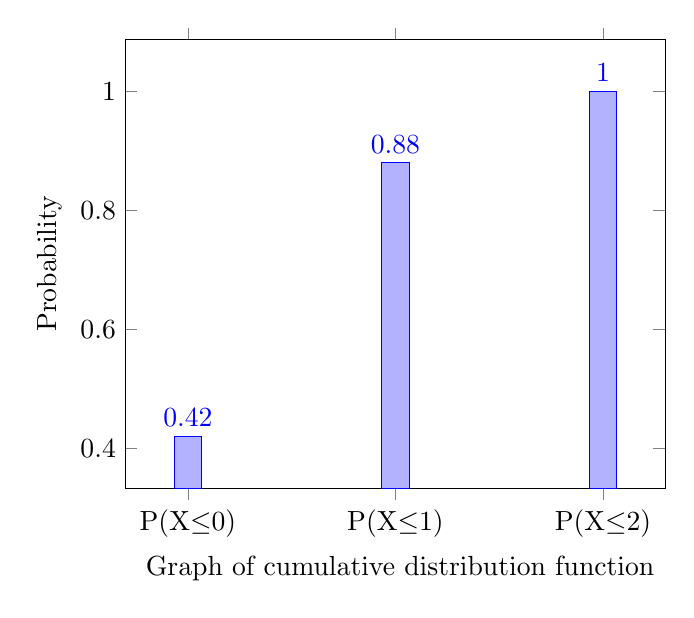
\begin{tikzpicture}

\begin{axis}
[
    ybar,
    enlargelimits=0.15,
    ylabel={Probability}, % the ylabel must precede a # symbol.
    xlabel={\ Graph of cumulative distribution function},
    symbolic x coords={P(X$\leq$0),P(X$\leq$1),P(X$\leq$2)}, % these are the specification of coordinates on the x-axis.
    xtick=data,
     nodes near coords, % this command is used to mention the y-axis points on the top of the particular bar.
    nodes near coords align={vertical},
    ]
\addplot coordinates {(P(X$\leq$0),0.42) (P(X$\leq$1),0.88) (P(X$\leq$2),1)};

\end{axis}
\end{tikzpicture}
\newpage
{\scshape } \hfill {\scshape DISCRETE STRUCTURES (CO1007) - Homework 06 - Probability} \hfill {\scshape }
 
\smallskip

\hrule

\bigskip

\bigskip 
\textbf{Problem 12. }[5 pts] Suppose that a Bayesian spam filter is trained on a set of 500 spam messages and 200
messages that are not spam. The word "exiting" appears in 40 spam messages and in 25 messages that are
not spam. Would an incoming message be rejected as spam if it contains the word "exiting" and the threshold
for rejecting spam is 0.9?
\bigskip

\textit{Solution}:

E: Spam message; F: the word “exciting” appears

p(E) = 5/7 : the probability of spam emails.

$p(\neg E) = 2/7$ : the probability of not spam emails.

\[p(F|E)=\frac{p(F\cap E)}{p(E)} = \frac{40}{500}=\frac{2}{25}\]

\[p(F|\neg E)=\frac{p(F\cap \neg E)}{p(\neg E)}=\frac{25}{200}=\frac{1}{8}\]

\[p(E|F)=\frac{p(F|E)\times p(E)}{p(F|E)\times p(E)+p(F\cap \neg E)\times p(\neg E)}=\frac{(2/25)\times (5/7)}{(2/25)\times (5/7)+(1/8)\times(2/7)}=\frac{8}{13} < 0.9\]

So the message containing the word "exiting" will not be rejected as spam.
%The probability of spam emails given that including “exiting” is  
%\[P(S|E) = \frac{P(S\cap E)}{P(E)} = \frac{8}{13}\]

%The probability of message be rejected as spam if it contains the word “exiting”
%: \[P(S|E) = \frac{8}{13} < 0.9\]
\newpage

{\scshape } \hfill {\scshape DISCRETE STRUCTURES (CO1007) - Homework 06 - Probability} \hfill {\scshape }
 
\smallskip

\hrule

\bigskip

\bigskip 
\textbf{Bonus Exercises: }

\textbf{7.1.2: }The probability that a fair die comes up six when
it is rolled is $\mathbf{\frac{1}{6}}$

\medskip

\textbf{7.1.6: }What is the probability that a card selected at random
from a standard deck of 52 cards is an ace or a heart?

There are 12 cards which are a heart and not an ace, 3 cards which are an ace and not a heart, and 1 card which is a heart and an ace.

$\Rightarrow$ The probability is $\frac{12+3+1}{52}=\mathbf{\frac{4}{13}}$
\medskip

\textbf{7.2.5}

With two dices, the combinations of the first and second dice to produce a sum of 7 are

(1,6),(2,5),(3,4),(4,3),(5,2),(6,1)

$\Rightarrow$ The probability is $\frac{1}{7}\times\frac{1}{7}+\frac{1}{7}\times\frac{1}{7}+\frac{1}{7}\times\frac{1}{7}+\frac{2}{7}\times\frac{2}{7}+\frac{1}{7}\times\frac{1}{7}+\frac{1}{7}\times\frac{1}{7}=\mathbf{\frac{9}{49}}$
\medskip

\textbf{7.3.2}

\[p(E|F)=\frac{p(E\cap F)}{p(F)}=\frac{p(F|E)*p(E)}{p(F)}=\frac{\frac{5}{8}\times\frac{2}{3}}{\frac{3}{4}}=\mathbf{\frac{5}{9}}\]

\textbf{7.3.8}

Let A: use opium, B: test positive .Given:

$P(B|\neg A) = 0.02, P(\neg B|A) = 0.05, P(A) = 0.01$

a. The probability that someone who tests negative
for opium use does not use opium: 
\[P(\neg A|\neg B)=\frac{P(\neg B|\neg A)\times P(\neg A)}{P(\neg B|\neg A)\times P(\neg A)+P(\neg B|A)\times P(A)}=\frac{(1-0.02)\times(1-0.01)}{(1-0.02)\times(1-0.01)+0.05\times0.01}\approx\mathbf{0.9995}\]

b. The probability that someone who tests positive
for opium use actually uses opium:

\[P(\neg A|\neg B)=\frac{P(B|A)\times P(A)}{P(B|A)\times P(A)+P(B|\neg A)\times P(\neg A)}=\frac{(1-0.05)\times0.01}{(1-0.05)\times0.01+0.02\times(1-0.01)}\approx\mathbf{0.3242}\]



\textbf{7.4.1}

Since the coin is unbiased, P(H) = 0.5
\[E(H)=(number\ of\ trials)\times P(H)=5\times\frac{1}{2}=\mathbf{2.5}\]

\textbf{7.4.5}

$P(X=3) =\frac{2}{7}$, $P(X=1)=P(X=2)=\dots=P(X=6)=\frac{1}{7}$ 

X is the number appear on the first die, Y is the number appear on the second die

E(X+Y) = E(X)+E(Y)

\[E(X)=E(Y)=1\times\frac{1}{7}+2\times\frac{1}{7}+3\times\frac{2}{7}+\dots+6\times\frac{1}{7}=\frac{24}{7}\]
\[E(X+Y)=\frac{24}{7}+\frac{24}{7}=\mathbf{\frac{48}{7}}\]

\end{document}